\documentclass[14pt]{article}

\usepackage[polish]{babel}
\usepackage[utf8]{inputenc}
\usepackage[T1]{fontenc}
\usepackage{extsizes}
\usepackage{graphicx}
\usepackage{tocloft}
\usepackage{amsmath}
\usepackage{multirow}
\usepackage{hyperref}


\font\titlefont=cmtt10 at 22pt

\title{
    
\includegraphics[scale=0.5]{images/logo-pwr-pion.png}
    \vspace{1cm}
    \\
    {\textbf{
    \titlefont Sygnały i obrazy cyfrowe
    \\ Laboratorium 3 - Demozaikowanie
    }}
}
    
\author{
    Informatyczne Systemy Automatyki
    \\
    \\ Wykonujący:
    \\ Igor Potyrała - 272518
    \\
    \\ Prowadzący - Przemysław Śliwiński
}
\date{Data laboratoriów: 22 listopada 2023}


\begin{document}
\maketitle
\newpage
% Spis treści
%\newpage
%\renewcommand{\cftsecleader}{\cftdotfill{\cftdotsep}}
%{
 % \hypersetup{linkcolor=black, hidelinks}
 % \tableofcontents
%}

% Wstęp teoretyczny, definicje
\section{Zadania}
\subsection{Cel zajęć}
Celem tych laboratoriów było zaimplementowanie demozaikowania, 
odtwarzając najpierw działanie matryc CMOS z filtrem kolorów 
Bayera oraz X-Trans, do wykonania zadania wykorzystałem także funkcję
interpolacji najbliższego sąsiada.


\subsection{Wyniki demozaikowania}
\vspace{1cm}
\begin{center}
    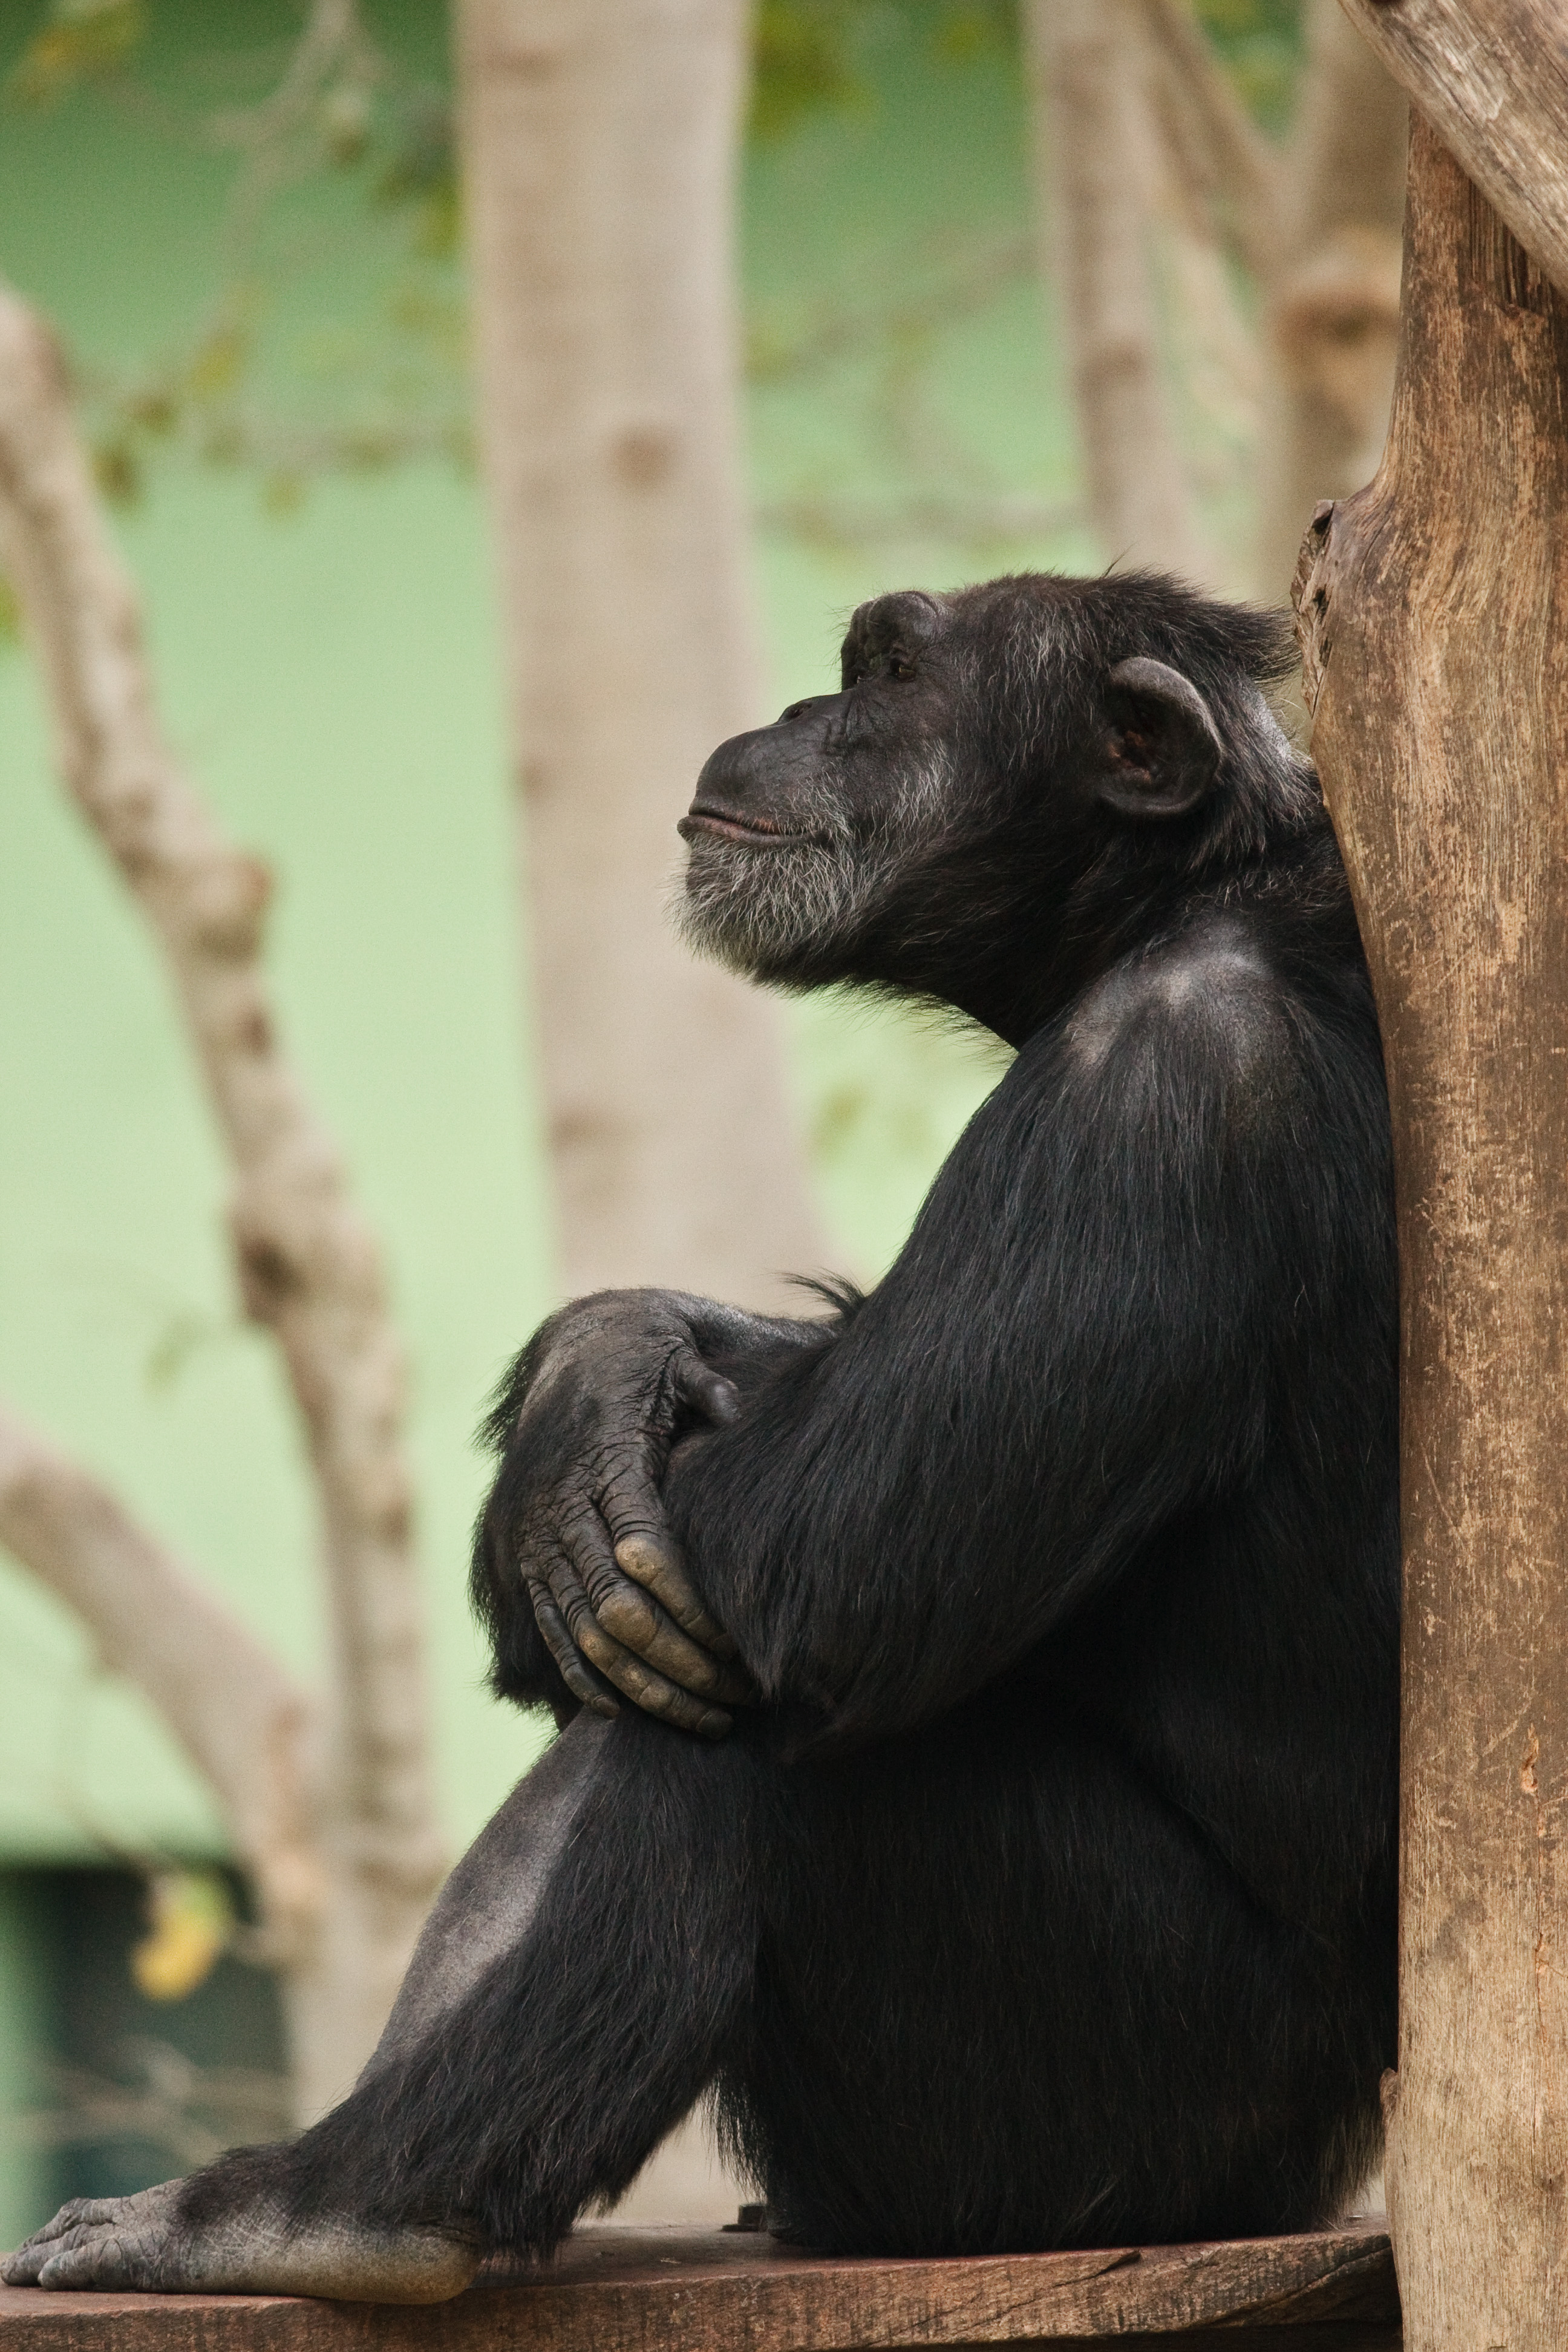
\includegraphics[scale=0.2]{images/Fella.jpg}
    \\ \small Obraz 1. Oryginalny.

    % BAYER
    \vspace{0.5cm}
    \includegraphics[scale=0.06]{images/Bayer.jpg}
    \\ \small Obraz 2. Po odtworzeniu matrycy Bayera.

    \vspace{0.5cm}
    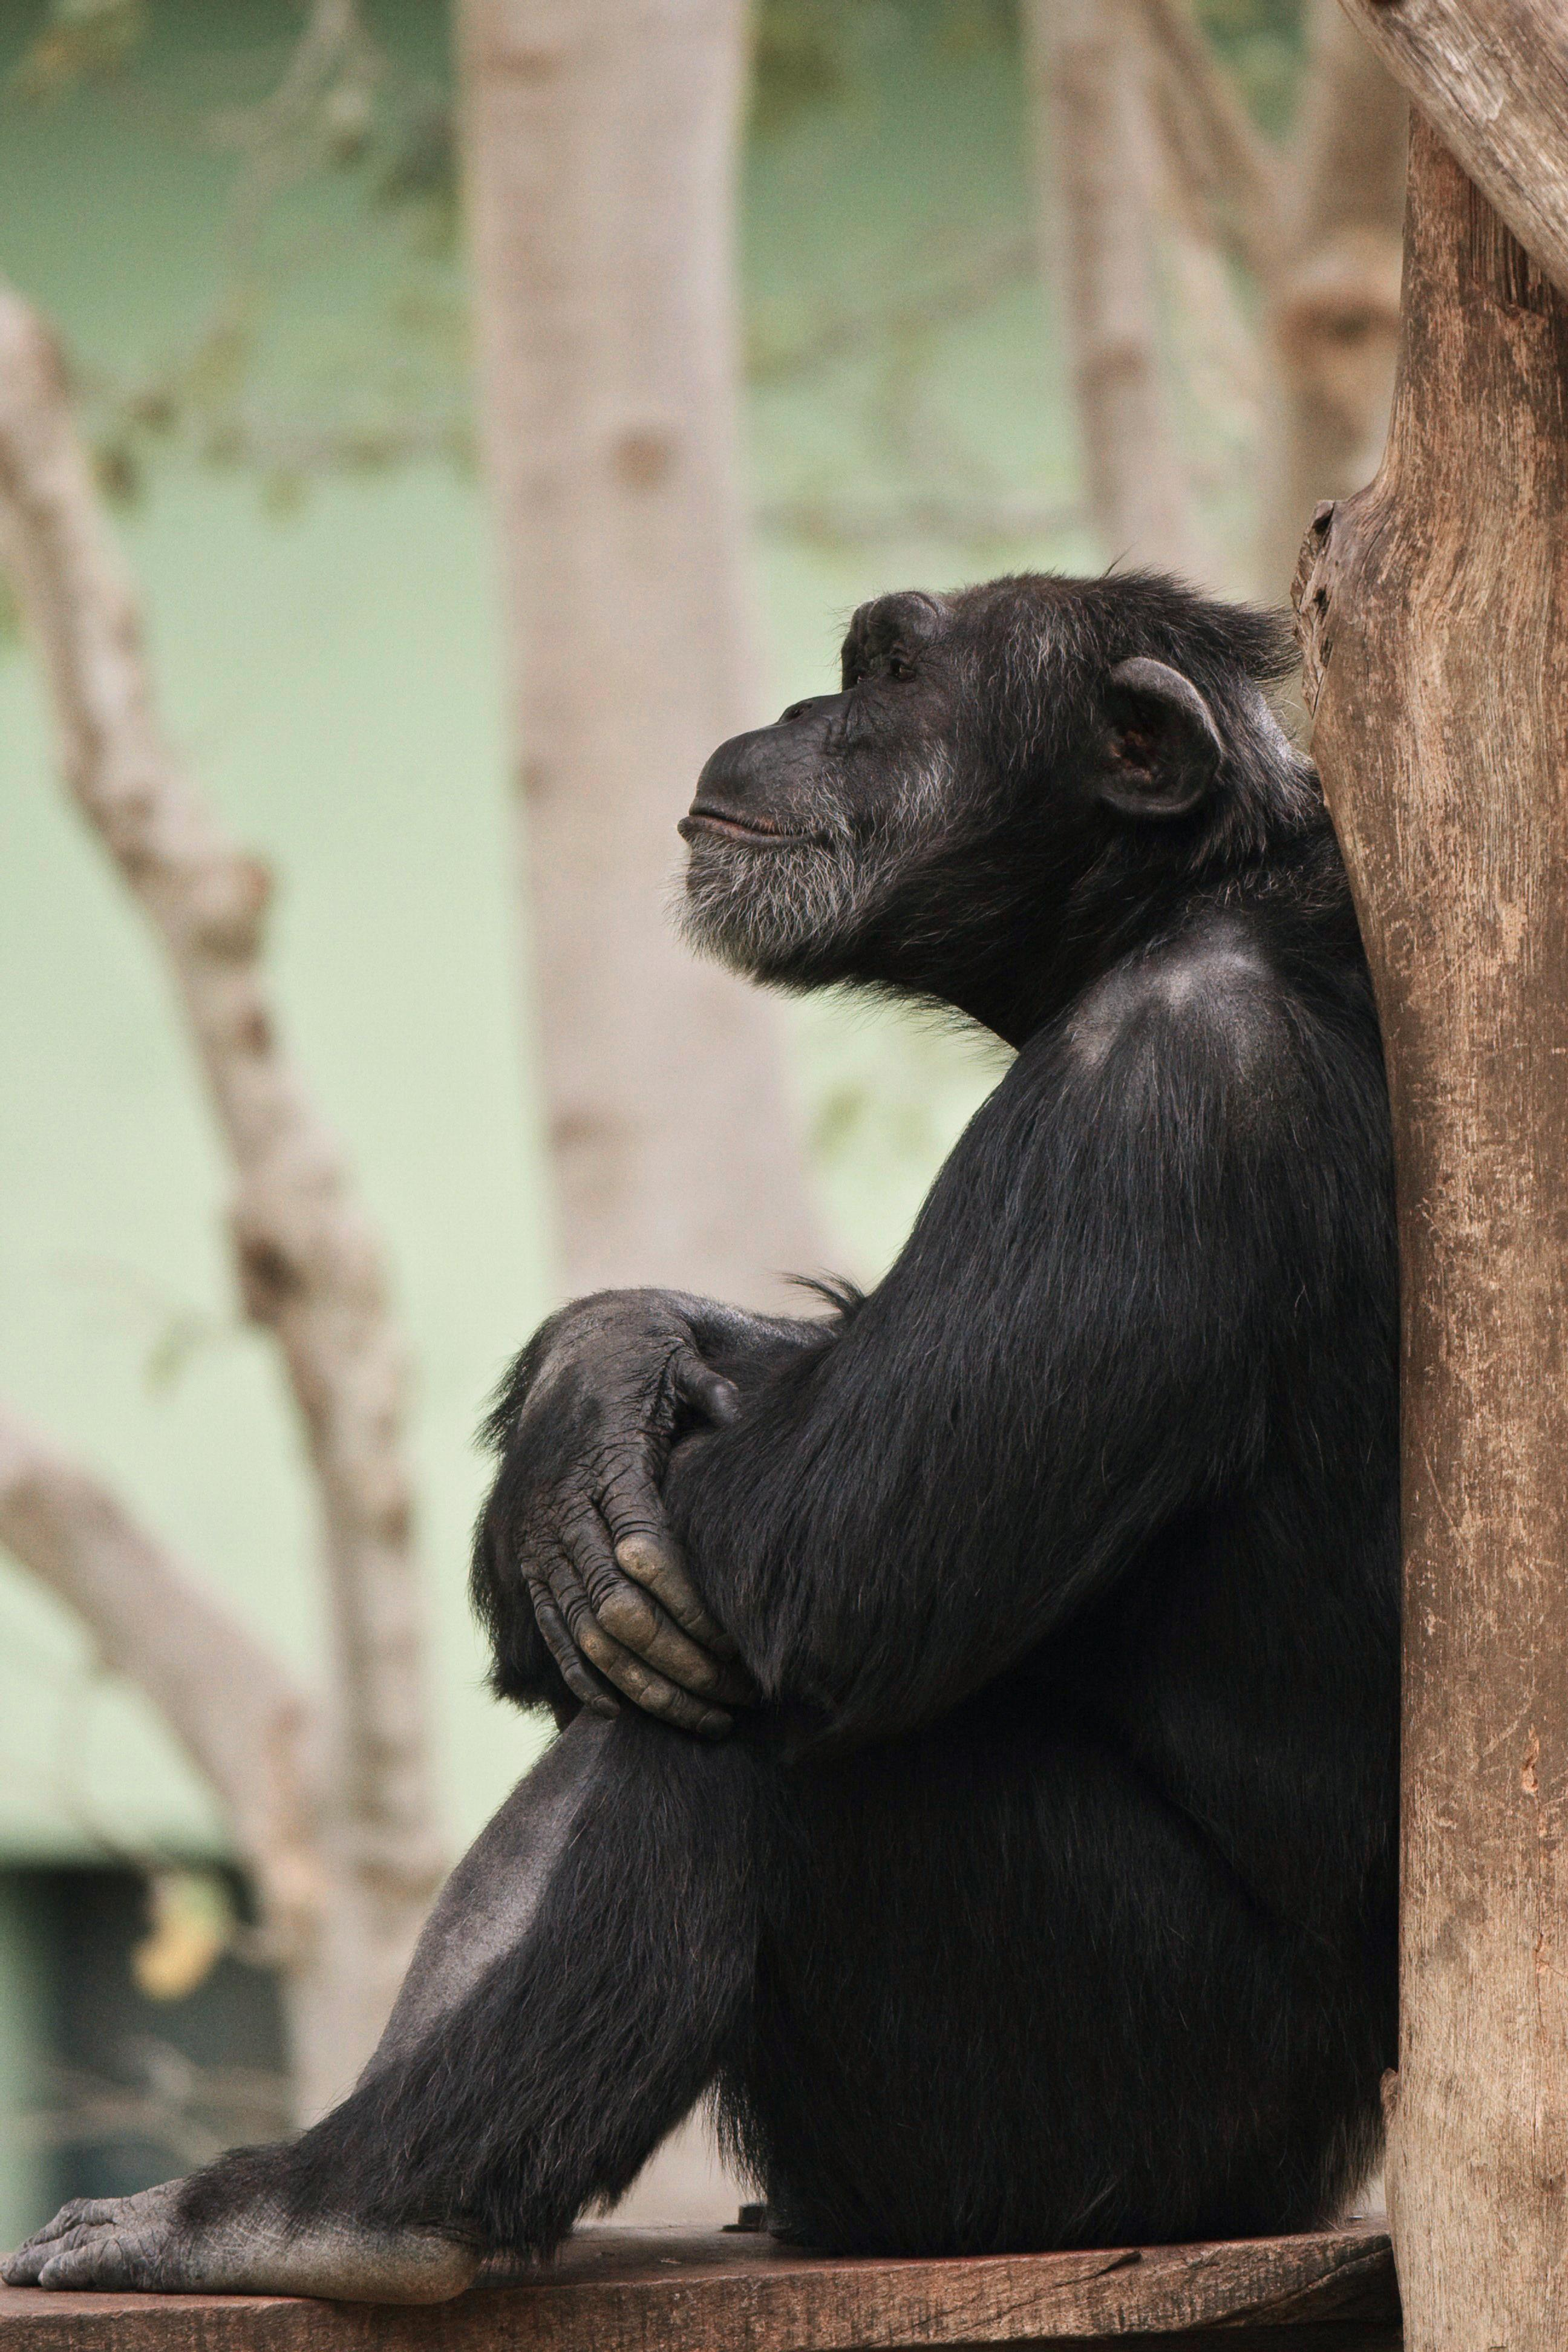
\includegraphics[scale=0.06]{images/Bayer_Demo.jpg}
    \\ \small Obraz 3. Po demozaikowaniu - Bayer.

    \vspace{0.5cm}
    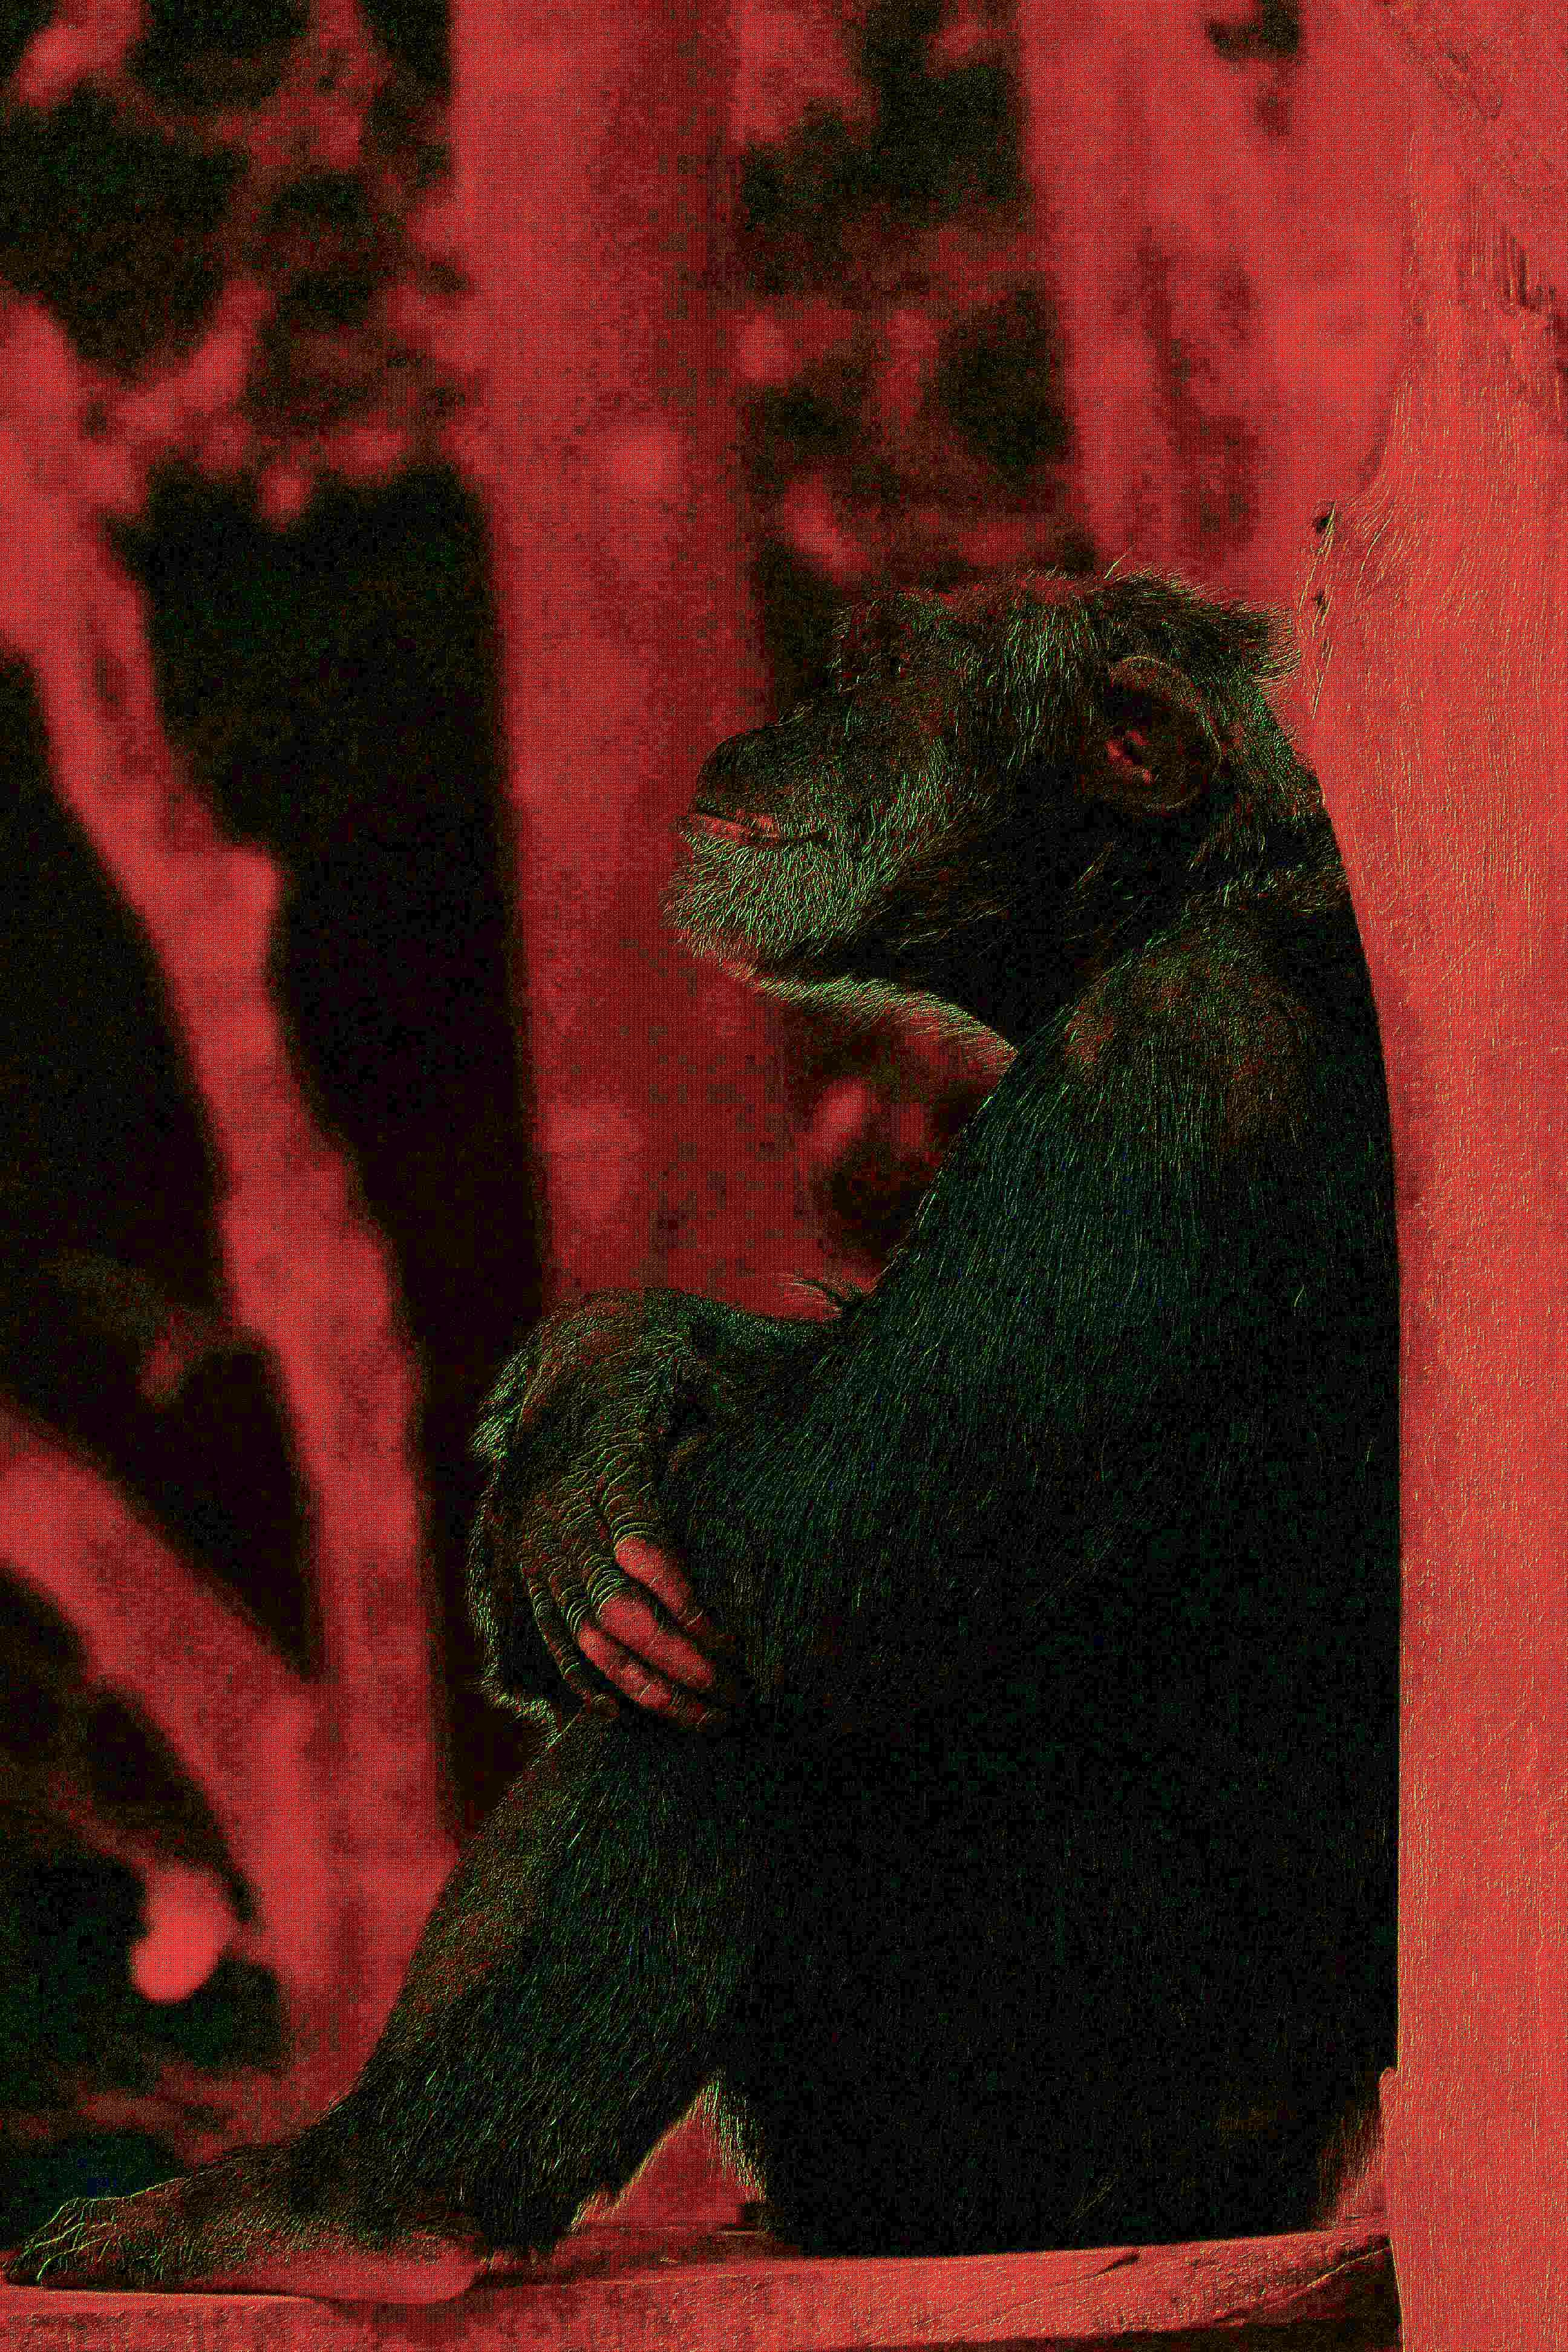
\includegraphics[scale=0.06]{images/Bayer_DIFF_br.jpg}
    \\ \small Obraz 4. Różnica między orygnalnym, 
    a zdemozaikowanym obrazem - Bayer.

    % XTRANS
    \vspace{0.5cm}
    \includegraphics[scale=0.06]{images/X_Trans.jpg}
    \\ \small Obraz 5. Po odtworzeniu matrycy X-Trans.

    \vspace{0.5cm}
    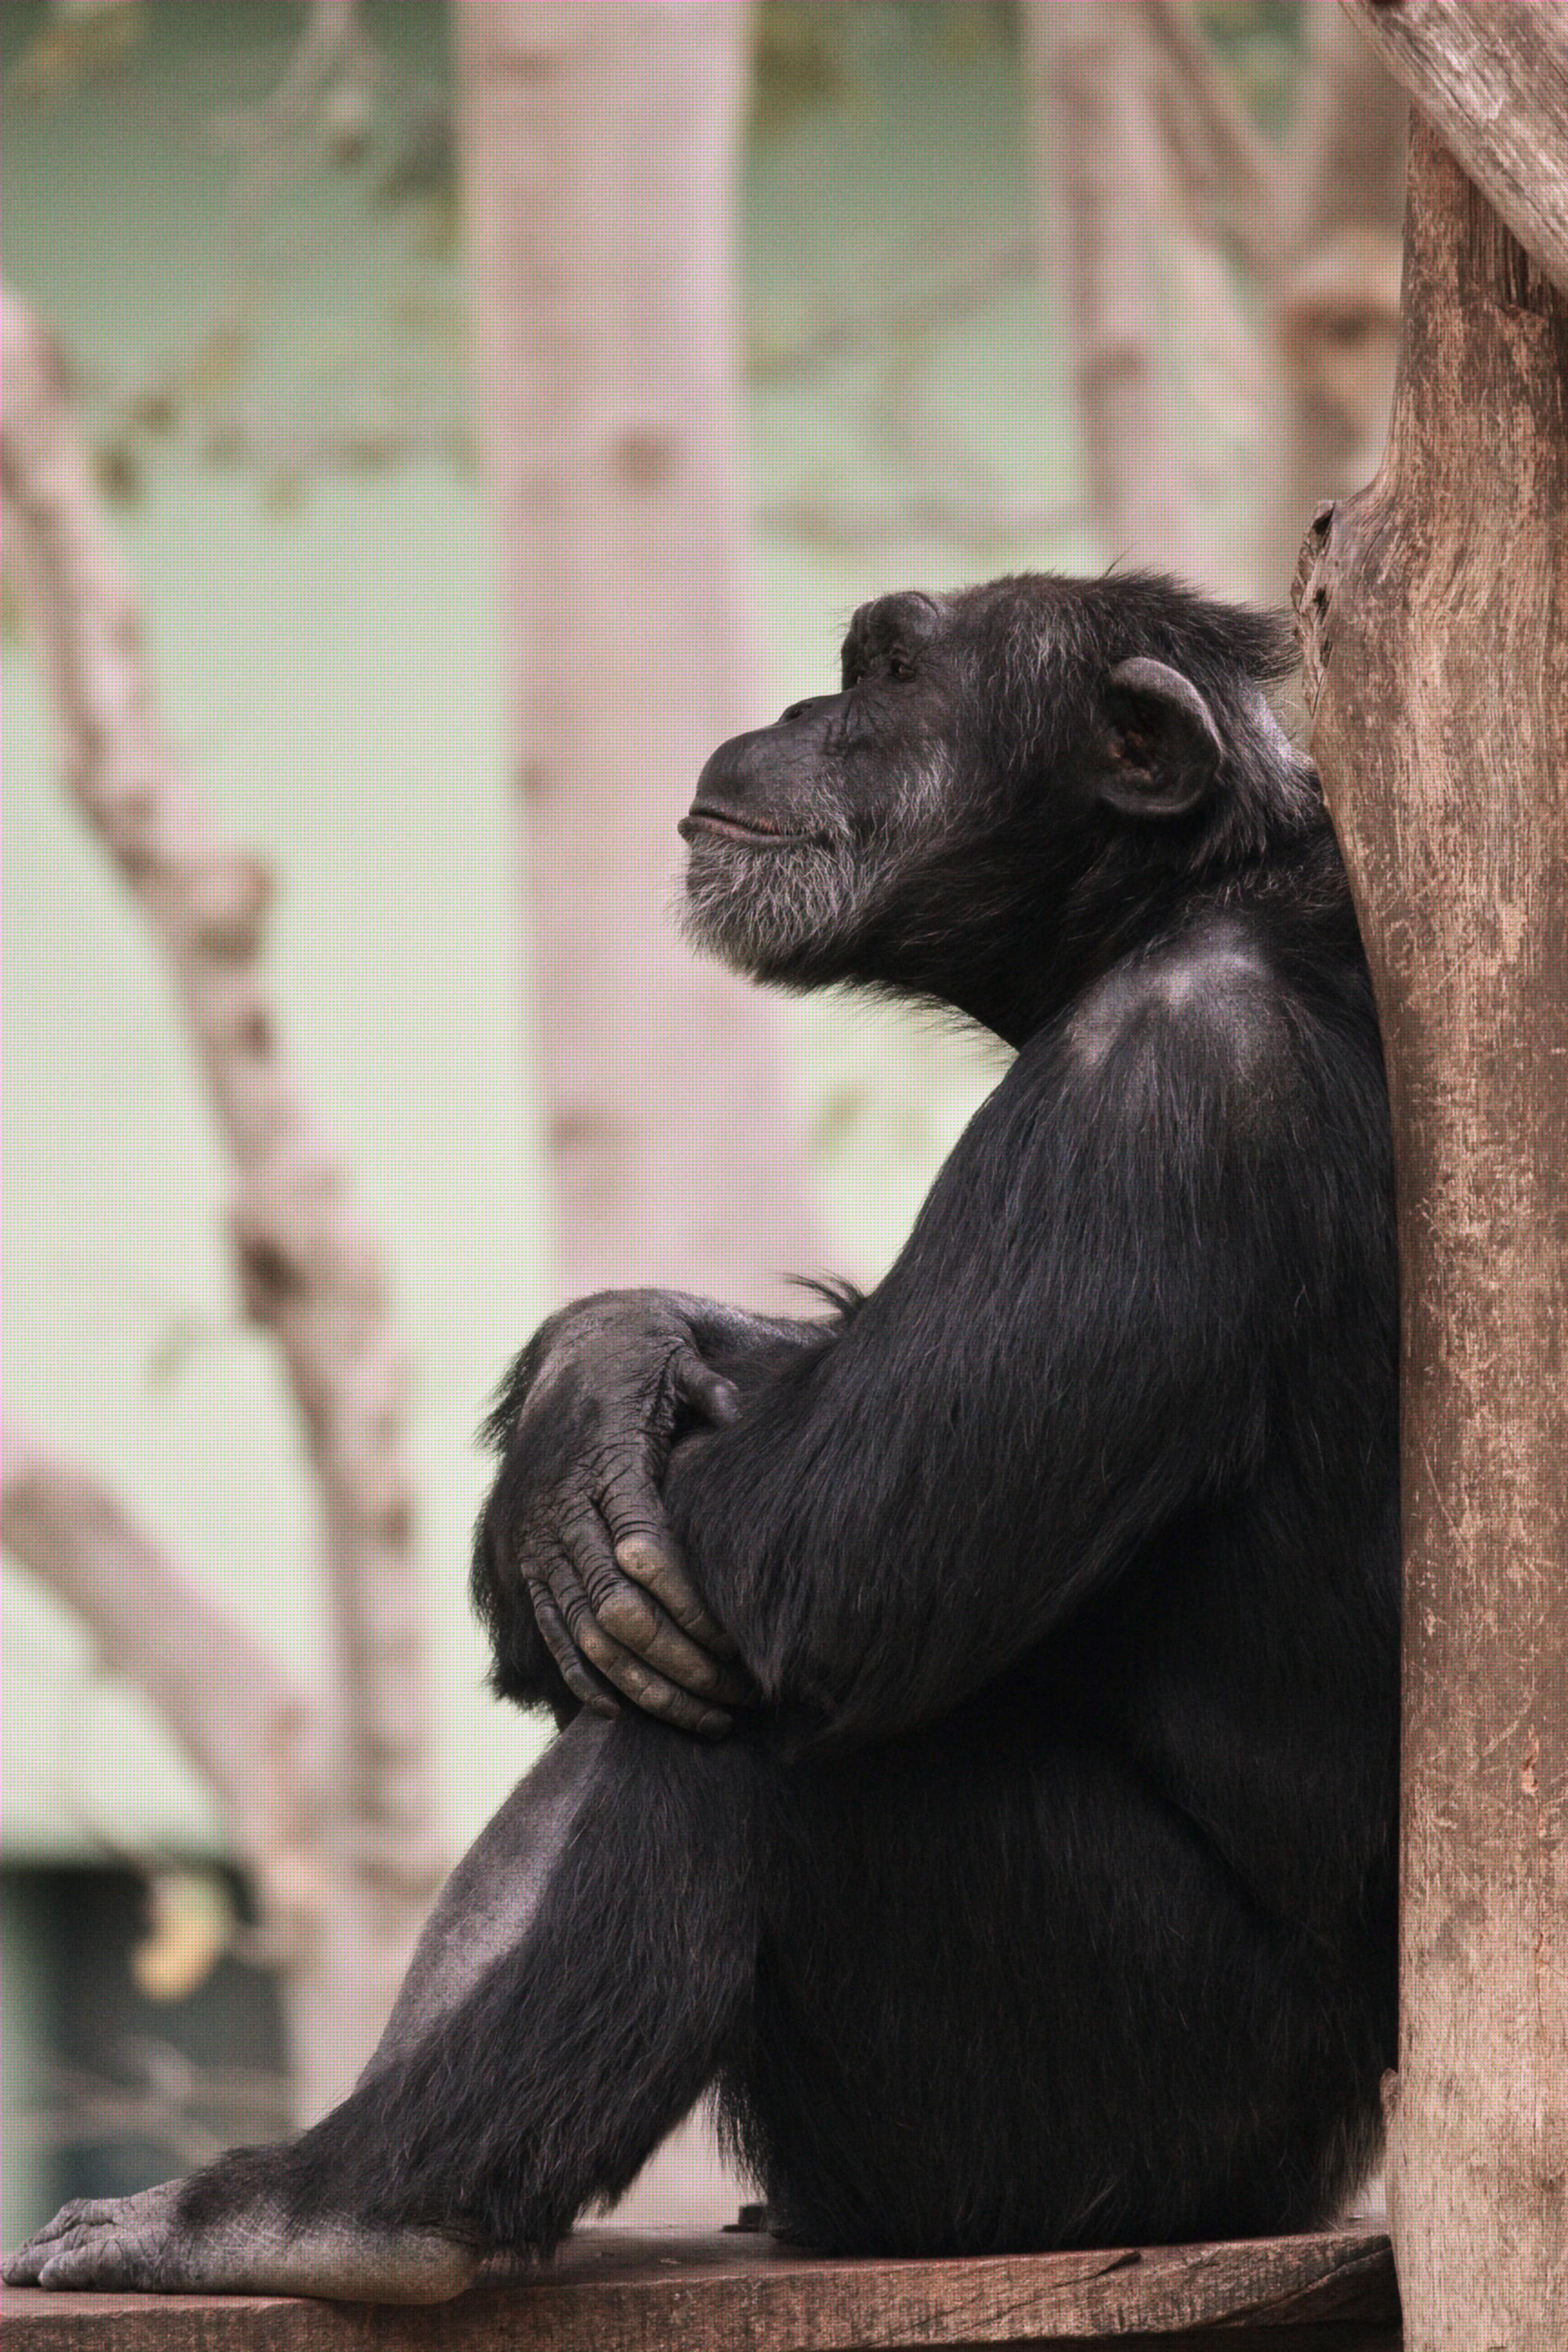
\includegraphics[scale=0.06]{images/X_Trans_Demo.jpg}
    \\ \small Obraz 6. Po demozaikowaniu - X-Trans.

    \vspace{0.5cm}
    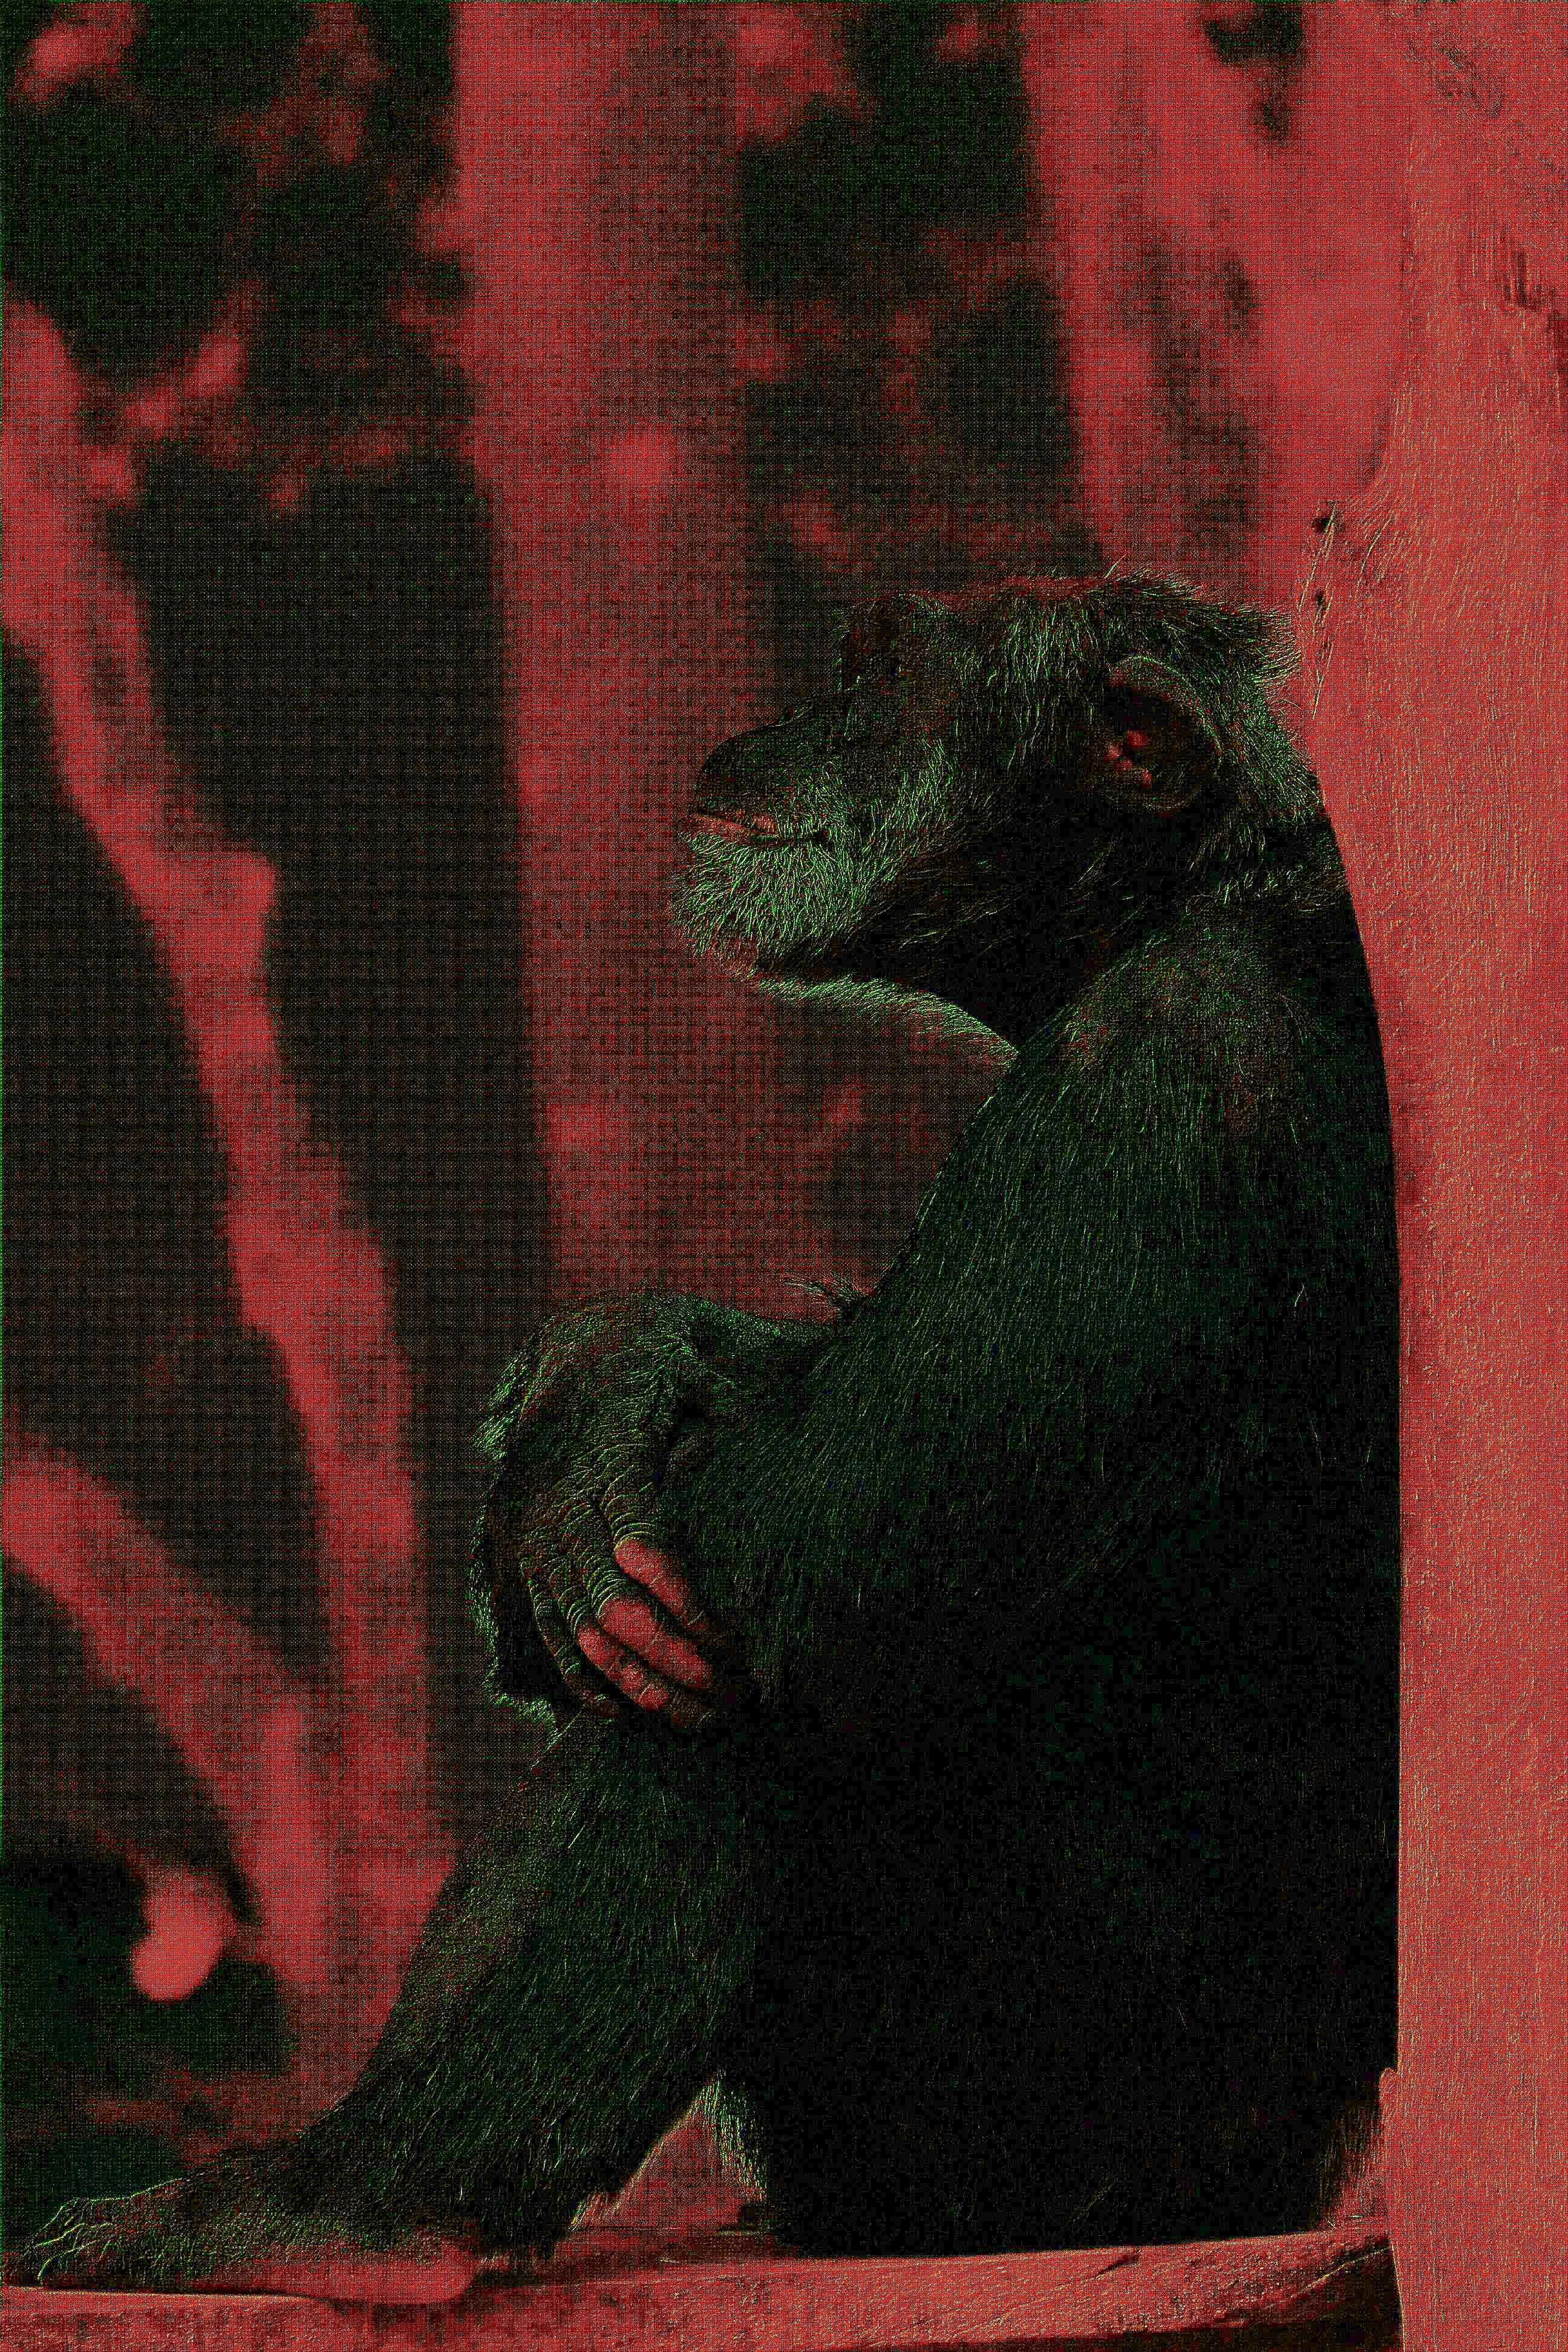
\includegraphics[scale=0.06]{images/XTRANS_DIFF_br.jpg}
    \\ \small Obraz 7. Różnica między orygnalnym, 
    a zdemozaikowanym obrazem - X-Trans.

    \vspace{1.5cm}
\end{center}

\newpage
\section{Wnioski}


\begin{center}
    Po zastosowaniu dla obu matryc interpolacji najbliższego sąsiada, wynika że o wiele
    lepiej wypadła matryca Bayera pod względem bliskości do 
    oryginalnego obrazu (niższy średni błąd kwadratowy). 




    \vspace{0.25cm}
    \begin{tabular}{|c|c|c|}
        \hline
        & Bayer & X-Trans  \\ \hline
        Błąd Średnio Kwadratowy & 43,53 & 60,96 \\ \hline
        Czas działania matryc & 0,28s & 9,5s \\ \hline
        Czas demozaikowania & 0,08s & 0,11s \\ \hline

    \end{tabular}
    \vspace{0.2cm}
    \\ \small Tabela 1. Przedstawiające charakterystyki 
    obrazów po demozaikowaniu dla matryc Bayera oraz X-Trans.
\end{center}

\end{document}